\documentclass{homework}
\usepackage{homework}
\usepackage{hanhua}
\title{report}
\subtitle{week 6}
\begin{document}

\maketitle
\section{lengthOfLastWord.h}
\subsection{函数说明}
输出字符串中最后一个单词的长度
\paragraph{输入}
一个字符串。
\paragraph{输出}
一个整形:最后一个单词的长度。
\paragraph{实现方法}
设置一个计数器和一个标志“单词中”状态的变量,从头依次读取字符:

每当读到非空白字符时,若未在“单词中”,即此时遇到了一个新的单词,将计数器清零后加一,并将状态设为“单词中”;若在“单词中”,则继续计数即可;

每当读到空白字符时,将状态设为不在“单词中”。

当读取完全部字符后,计数器中储存的就是最后一个单词的长度。
\subsection{复杂度}
\paragraph{时间复杂度}
$\mathcal{O}(n) ~ n$为字符串长度
\paragraph{空间复杂度}
$\mathcal{O}(1)$
\subsection{边界情况}
\begin{itemize}
    \item 传入NULL或空字符串“”将得到0;
    \item 传入字符串长度超过整型最大值将得到错误的结果。
\end{itemize}
\subsection{程序运行结果}
\begin{figure}[H]
    \centering
    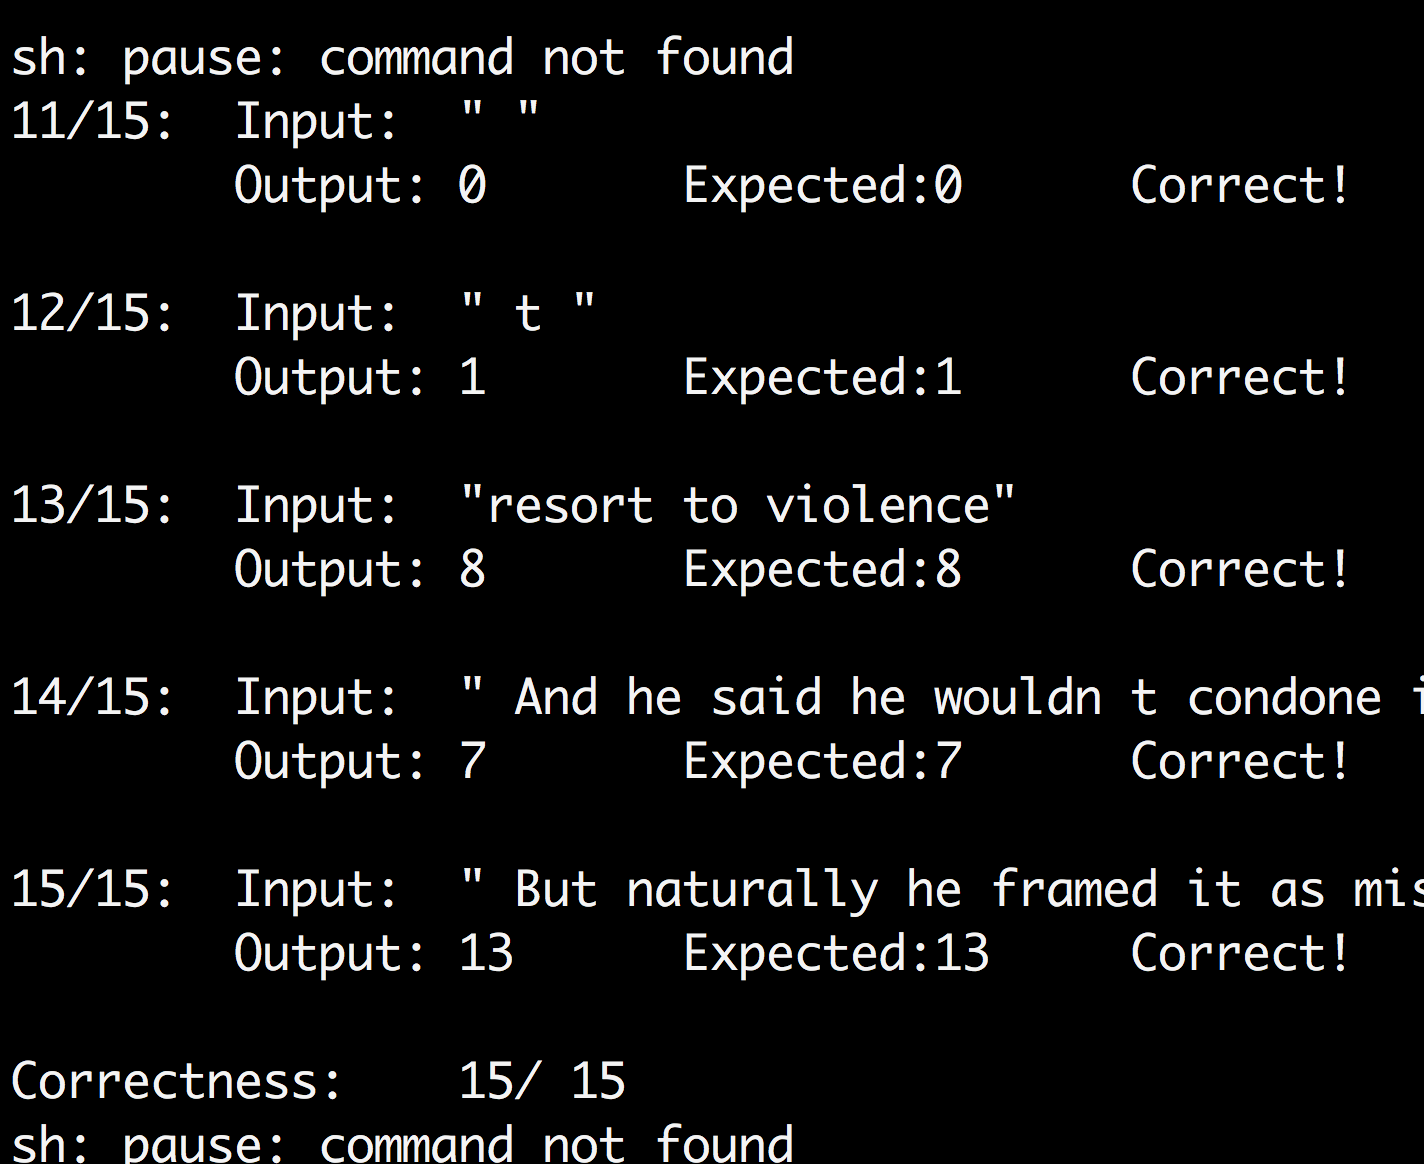
\includegraphics[width=7cm]{lol.png}
\end{figure}
\section{wordPattern.h}
\subsection{函数说明}
判断字符串是否符合样式规则,即可建立样式中字母到字符串中单词的保序的一一映射。
\paragraph{输入}
一个仅含有小写字母的字符串:样式规则,和一个用单空格分隔的仅含小写字母单词的字符串。
\paragraph{输出}
一个伪布尔值,表示字符串是(1)/否(0)符合样式规则。
\paragraph{实现方法}
\paragraph{第一步:}检查是否存在样式到单词的映射,即同样的样式必指向同样的单词。

首先,对于样式中的每个字母,找到在样式中第一次出现该字母的位置。

然后,在字符串中每遇到一个新的单词,记录其起始位置,若其对应样式第一次出现,则直接跳到下一个单词;

若出现过该样式(第一次出现该样式的位置不是自己),则将其与其对应位置的样式字母第一次出现的样式位置所对应的单词进行比对:若不一样则返回false。

若出现单词数量大于或小于样式长度,返回false。
\paragraph{第二步:}检查映射是否为单射,即同样的单词也拥有同样的样式字母。
对于每个单词,将其与之前的所有单词进行比对,若遇到一样的单词,检查其对应样式字母是否一样,若不一样则返回false。

若通过了前两步测试,则返回true。
\subsection{复杂度}
\paragraph{时间复杂度}
$\mathcal{O}(p^2+s+s^2)=\mathcal{O}(p^2+s^2) ~ $其中p为样式长度,s为字符串长度。

$p^2$为构建寻找相同样式位置所需时间,$s$为检查映射时间,$s^2$为检查单射时间。
\paragraph{空间复杂度}
$\mathcal{O}(p+s)$

p为记录样式字母首次出现位置所需空间,s为记录每个单词的初始位置所需空间。
\subsection{边界情况}
\begin{itemize}
    \item 若样式和字符串都为NULL,或其中一个为NULL另一个为空字符串“”,则返回true;
    \item 若样式和字符串其中一个为NULL但另一个不是空字符串“”,则返回false;
    \item 支持在第一个单词前/最后一个单词后增加空白符;
    \item 支持多个空格和制表符作为分隔;
    \item 但如果字符串中只有空白(但非空字符串)而传入样式是NULL会返回false,但应为true;
    \item 提交的程序抑制了所有报错信息。
\end{itemize}
\subsection{程序运行结果}
\begin{figure}[H]
    \centering
    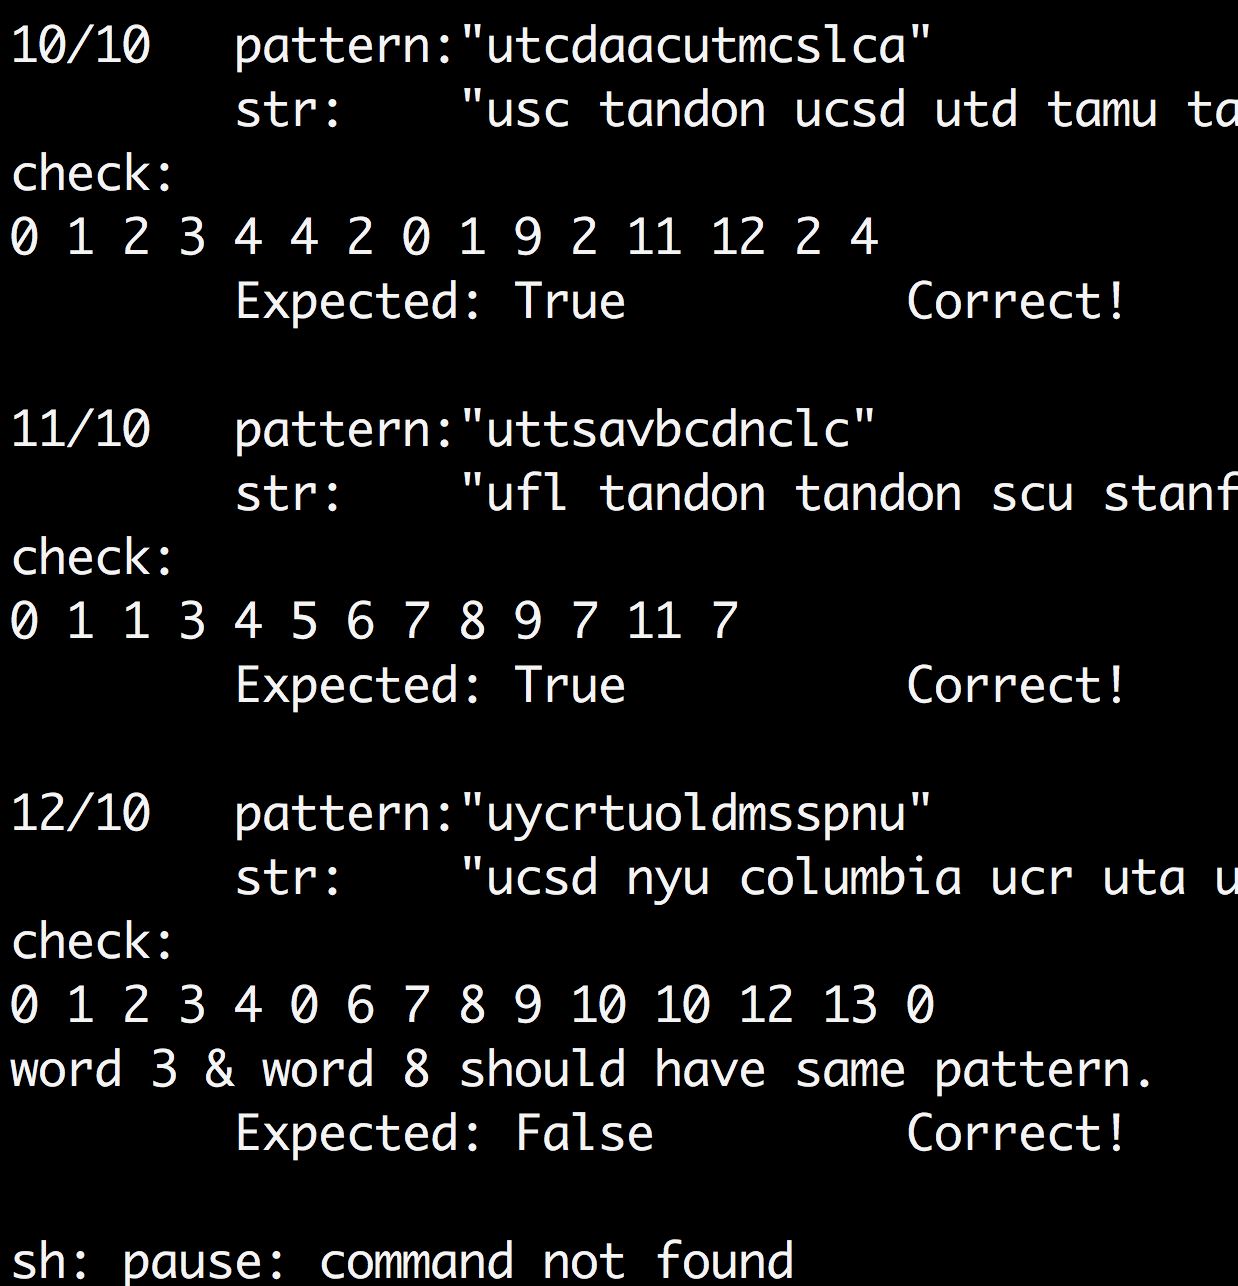
\includegraphics[width=7cm]{wp.png}
\end{figure}
\end{document}
